% \cfoot[{\thepage\ of \pageref*{LastPage}}]{\thepage\ of \pageref*{LastPage}} 
\section{Introduction}
\pagestyle{headings}


\subsection{system biology}
System biology is there for the extraction of a system wide understanding of living organismen. This includes the interaction of multiple proteins, genes, metabolits et cetera, which are measured in the laboratory. This approach gets more significant in the analysis of executed omics experiments which easily results in data in the gigabyte range (Zitieren: Toward an integrated ...). Mathematical modeling has proven to be a promising tool for the study of the complex processes of environmental stress adaptation, to reveal the role of each biological component in the system and to reveal  how the system level properties emerged from collected activites of individual components \cite{Ke_2013}. \\\\
Currently limitations of the system biology approach are the usages and constructions of mathematical equations which should represent the biological system. This is a trade off between reduction of the system of interest without dimishing the quality of the information value or reasonableness intended digital twin. Another important problem is that there does not exists a complete biological understanding and knowledge of all system component. The system biological appproach is therefore only a heuristic approach (zitieren!!!) \\\\
In-depth insights of an investigated system are e.g. useful for medicine and the biotechnology sector (cite: Toward an integrated software platform for systems pharmacology!!!!) because this results in the improvement of  
well constructed mathematical models of a cell system could be useful for the design of target-oriented medications. \\\\
An increase in external osmolarity leads to a cell volume reduction. The cell counteract this high osmotic pressure by increased intracellular glycerol as an osmolyte and restores in this way its volume. \\


Mathematical models \textit{in silico} are further helpful to test laboratory experiments \textit{in silico} to identify meaningful experiments by construction of DoE (Design of Experiment). This helps to save the resources (e.g. money, time) of the experimentalist and could results in a deeper understanding of the underlying biological system.\\\\

\subsection{Saccharomyces cerevisiae}
The yeast Saccharomyces cerevisiae (\emph{S. cerevisiae}) is a unicellular eucaryotic organism and belongs to the class of fungi \cite{Feyder2015}. It was the first eucaryotic organism where the whole genome had been full sequenced. \cite{goffeau1996life}. \emph{S. cerevisiae} is one of the beast characterized eukaryotic models \cite{Feyder2015}.\\\\
In nature, the environment of S. cerevisiae varies in factors like temperatur, nutrient levels or osmolarity with the time and the cell must adapt with these changes. \cite{JannisUhlendorf} The Hog-Pahtway in yeast has a significant role in the adaption process after an osmotic stress exposure. It normalize the volume of the cell and with that the water balance with an accumulation of the osmolyt glycerol inside, by closing the glycerol membran transporter Fps1 (\cite{Saito2012},  \cite{ASimpleMathematicalModel}) and the production of glycerol.  

\subsection{state of the art}
It already exists multiple models for the hog pathway (signaling module), ion transport (transport module) and the volume regulation (volume module) (!!! alles hier noch mit Zitaten belegen). The signaling module keeps tracks of the stress response signaling pathways \\
Each of these models describe a part of the cell system while assuming other important aspects of the system as constant (see picture \ref{IntersectionsOfTheModels}).

\begin{figure}[h!]
	\begin{center}
		\begin{minipage}{0,8\textwidth}
			
			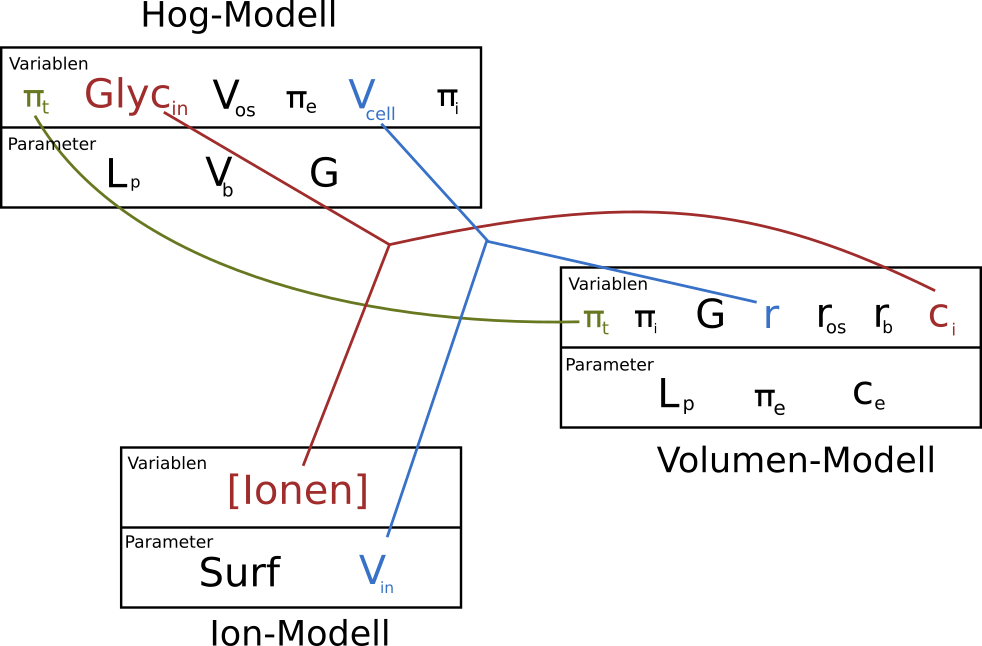
\includegraphics[width=\textwidth]{picture/model_intersections.png}
			\caption{intersections of the three models } 
			\label{IntersectionsOfTheModels} 
		\end{minipage}
	\end{center}
\end{figure}

In our momentan state of knowledge, there is not yet a model which integrate this three modules into a single model. The combined model simulates the interaction between extra- and intracellular ionconcentration, changes in cell volume and the activity of the MAP cascade (???). The model senses the differences in the osmolarity between the cell and its environment and adapt with the important high osmolarity glycerol (HOG) signaling pathway with the MAP cascade the cell volume and the intracellular osmolyt concentrations. 

\subsection{theory of the used models}
\subsubsection{ion model}
Per diffiniton, osmolarity means the amount of substance $n$ of osmotic activ particles per volume $V$ of the solution. Osmotic pressure accurs if two solutions with different osmolarity are seperated by a semipermeable membrane, where not all substances can pass the membrane for creating an equilibrium.\\
S. cerevisiae has a plasma membrane which functions as a semipermeable membrane. Water can diffuse freely through it, to adapt to the osmotic changes. At a hyperosmotic shock in the extracellular environment, water will flow out of the cell and let the cell shrink in volume. Cause of the shock event the high osmolarity glycerol (HOG) pathway in S. cerevisiae gets activ and synthesis the osmolyte glycerol. With that the cell increases the internal osmolarity and restores it’s volume cause of the influx of water.\\\\
The immediate effect on yeast to an osmotic shock involves water outflow and decreasing volume \cite{ASimpleMathematicalModel}.\\
The ion model consists out of a non-equivilibrium thermodynamic (NET) approach to model the transport of the ion over the plasma membrane. NET is the analysis of spartial inhomogeneous systems and of time dependent processes. It is not valid if there are very fast processes or big inhomogeneity. The ion model assumes that both compartimens are well mixed. This way the NET approach hold true. \\
Fluxes over membranes are irreversible processes. This will lead to a production of entropy in the system, which is calculated by the entropy production density $\sigma$ which is respresented with the equation \ref{EntropyProductionDensity}

\begin{equation}\label{EntropyProductionDensity}
	\sigma = \vec{J_Q}\left(\frac{1}{T}\right) - \sum_{i=1}^{k}\vec{J_{c_i}}grad \left(\frac{\eta _i}{T}\right) + \sum_{r=1}^{R}J_r \frac{A_r}{T} \geq 0
\end{equation}
Equation \ref{EntropyProductionDensity} summeries the production of entropy under the conditions of temperatur difference, concentration difference and chemical reactions.
Fundamentally, $\sigma$ can only be created by fluxes $J$ with it’s forces $X$. In the area around equilibrium we can further assume that a flux $J$ is linearly coupled over a phenomenological coefficient $L$ with it’s forces $X$, because at equilibrium all forces and fluxes vanish. Under this condition the following statement holds true.
\begin{equation}\label{stoeachimetricCoeff}
	\sigma = \sum_{i}J_i X_i =\sum_{i}\sum_{j}L_{ij}X_j X_i
\end{equation}
After some other assumption made from the ion model (for deeper insight see \cite{Gerber_2016}), the equation for the flux of ion k is:
\begin{equation*}
J_k = \sum_{j=1}^n L_{kj}(RT\cdot ln\left(\frac{c_k^{in}}{c_k^{out}}\right) + z_kF\Delta \phi ) + L_{kAr}A_{Ar}
\end{equation*}
In the ion model a glycerol stimulus is further simulated. Ion regulation determines many physiological parameters, such as cell volume \cite{Ke_2013}.\\\\
\subsubsection{volume model}
Turgor pressure prevents exaggerated swelling and maintains cell shape \cite{volumeModel}. The volume model \cite{volumeModel} describes the water flux $J_w$ between the cell and the environment with 
\begin{equation}\label{waterFlux}
	J_{w} = - \frac{d}{dt} V_{os} = G * Lp * (\pi_e + \pi_t - \pi_i)
\end{equation}
with $Lp$ as the hydraulic conductivity, $G$ the cell surface and the internal, external and turgor pressure  ($\pi_i$, $\pi_e$ , $\pi_t$). The volume model only holds true for a individual yeast cell in G1 phase \cite{volumeModel}.
The cell volume depends essential on the relation of the internal, external and turgor pressure. The internal and external pressure $\pi$ depends on the concentration $c$ of the osmotic active substance in the corresponding areas correlated over the equation \ref{osmotic_pressure}
\begin{equation} \label{osmotic_pressure}
	\pi = c \cdot R \cdot T	
\end{equation} 

\subsubsection{hog model}
The hog model is composed out of the Hog1 Mitogen Activated Protein Kinase (MAPK) cascade. This cascade is conserved even in higher eukaryotes including humans (\cite{ASimpleMathematicalModel}). The Hog1 MAPK is activated in the response to an increase in extracellular osmolarity \cite{Saito2012}. All other non-osmotic stresses (e.g. temperature stres \cite{Saito2012}) which are known to also activate the HOG pathway are not represented in this model. The MAPK pathways are important for transmitting and processing signals from the cell membran into the cell \cite{ASimpleMathematicalModel}. \\
Hog1n MAPK is activated by the upstream Pbs2 MAP kinase kinase (MAPKK) by phosphorylation. 


\newpage